\documentclass{../../../oss-ap12ibhl-print}

\begin{document}
\genheader

\gentitle{5}{CIRCULAR MOTION AND GRAVITY}

\begin{questions}
  
  \question A \SI{1000}{\kilo\gram} car experiences a centripetal force of
  \SI{1.8e5}{\newton} while making a turn. The car is moving at a constant
  speed of \SI{30}{\metre\per\second}. What is the radius of the turn?
  \begin{choices}
    \choice\SI{.2}{\metre}
    \choice\SI{1}{\metre}
    \choice\SI{2}{\metre}
    \choice\SI{4}{\metre}
    \choice\SI{5}{\metre}
  \end{choices}

  \question A record player has four coins at different distances from the
  center of rotation. Coin A is 1 cm away, Coin B is 2 cm away, Coin C is 4 cm
  away, and Coin D is 8 cm away. If the player is spinning 45 rotations/min,
  what coin has the greatest tangential velocity?
  \begin{choices}
    \choice Coin A
    \choice Coin B
    \choice Coin C
    \choice Coin D
    \choice All the coins have equal tangential velocities.
  \end{choices}

  \question Friction allows a car to make a turn at a speed of 10 miles per
  hour. By what factor will the friction have to change to allow the driver to
  make the same turn at twice the speed?
  \begin{choices}
    \choice Four times the friction
    \choice Twice the friction
    \choice The same amount of friction
    \choice One-half the friction
    \choice One-fourth the friction
  \end{choices}

  \question A tetherball is whirled in a horizontal circle above your head. If
  the string breaks, the ball will follow what type of path if it is observed
  from above?
  \begin{choices}
    \choice Straight outward from the center
    \choice Straight toward the center
    \choice An expanding spiral
    \choice A curved path that gradually approaches a straight line
    \choice Tangent to the original circular path
  \end{choices}

  \question A pendulum bob is attached to a string that is tied to the ceiling,
  and the bob is pulled back and released. As the bob moves through the bottom
  of the swing, how does the magnitude of the tension force from the string
  compare to the gravitational force on the bob?
  \begin{choices}
    \choice The tension force is less than the gravitational force.
    \choice The tension force is greater than the gravitational force.
    \choice The tension force is equal to the gravitational force.
    \choice The mass of the ball is needed in order to compare these forces.
    \choice The release height of the ball is needed in order to compare these
    forces.
  \end{choices}

  \question A pendulum bob is attached to a string that is tied to the ceiling,
  and the bob is pulled back and released from different heights. As the bob
  moves through the bottom of the swing, how is its centripetal acceleration
  related to its speed?
  \begin{choices}
    \choice The centripetal acceleration is directly proportional to the speed
    of the pendulum.
    \choice The centripetal acceleration is inversely proportional to the speed
    of the pendulum.
    \choice The centripetal acceleration is directly proportional to the square
    of the speed of the pendulum.
    \choice The centripetal acceleration is inversely proportional to the square
    of the speed of the pendulum.
    \choice There is no relationship between the centripetal acceleration and
    the speed.
  \end{choices}
  \vspace{.7in}
  
  \question Two satellites of equal mass orbit a planet. Satellite B orbits at
  twice the orbital radius of Satellite A. Which of the following statements is
  true?
  \begin{choices}
    \choice The gravitational force on Satellite A is four times less than that
    on Satellite B.
    \choice The gravitational force on Satellite A is two times less than that
    on Satellite B.
    \choice The gravitational force on the satellites is equal.
    \choice The gravitational force on Satellite A is two times greater than
    that on Satellite B.
    \choice The gravitational force on Satellite A is four times greater than
    that on Satellite B.
  \end{choices}
    
  \question A proposed ``space elevator'' can lift a \SI{1000}{\kilo\gram}
  payload to an orbit of \SI{150}{\kilo\metre} above the Earth's surface. The
  radius of the Earth is \SI{6.4e6}{\metre}, and the Earth's mass is
  \SI{6.e24}{\kilo\gram}. What is the gravitational potential energy of the
  payload when it reaches orbit?
  \begin{choices}
    \choice\SI{-1.0e3}{\joule}
    \choice\SI{-2.7e6}{\joule}
    \choice\SI{-6.1e10}{\joule}
    \choice\SI{-2.7e12}{\joule}
    \choice\SI{-1.0e15}{\joule}
  \end{choices}

  \uplevel{
    \textbf{Questions \ref{centrifugal1}--\ref{centrifugal2}} are based on the
    following graph:
    \cpic{.45}{a-graph}
  }
  
  \question Engineers have designed a centrifuge for studying the effects of
  high gravity environments on plants and animals. This graph shows the results
  of the relationship between the radius and the centripetal acceleration. If
  the scientists want to simulate a ``3-G environment,'' then what should the
  radius of the centrifuge be?
  \label{centrifugal1}
  \begin{choices}
    \choice 1 m
    \choice 2 m
    \choice 3 m
    \choice 5 m
    \choice 10 m
  \end{choices}
    
  \question If an astronaut with a mass of 70 kg were placed in that centrifuge
  with a radius of 5 m, what would be the centripetal force acting on him?
  \label{centrifugal2}
  \begin{choices}
    \choice 300 N
    \choice 700 N
    \choice 1400 N
    \choice 2100 N
    \choice 2400 N
  \end{choices}
  \newpage
  
  \question A satellite orbits the Earth at a distance of
  \SI{200}{\kilo\metre}. If the mass of the Earth is \SI{6.e24}{\kilo\gram} and
  the Earth's radius is \SI{6.4e6}{\metre}, what is the satellite's speed?
  \begin{choices}
    \choice\SI{1.e3}{\metre\per\second}
    \choice\SI{3.5e3}{\metre\per\second}
    \choice\SI{7.8e3}{\metre\per\second}
    \choice\SI{5e6}{\metre\per\second}
    \choice\SI{6.1e7}{\metre\per\second}
  \end{choices}
    
  \question When climbing from sea level to the top of Mount Everest, a hiker
  changes elevation by \SI{8848}{\metre}. By what percentage will the
  gravitational field of the Earth change during the climb? (The Earth's mass
  is \SI{6.e24}{\kilo\gram}, and its radius is \SI{6.4e6}{\metre}.)
  \begin{choices}
    \choice It will increase by approximately \SI{.3}{\percent}.
    \choice It will decrease by approximately \SI{.3}{\percent}.
    \choice It will increase by approximately \SI{12}{\percent}.
    \choice It will decrease by approximately \SI{12}{\percent}.
    \choice The gravitational field strength will not change.
  \end{choices}

  \question Four planets, A through D, orbit the same star. The relative masses
  and distances from the star for each planet are shown in the table. For
  example, Planet A has twice the mass of Planet B, and Planet D has three
  times the orbital radius of Planet A. Which planet has the highest
  gravitational attraction to the star?
  \begin{center}
    \vspace{-.1in}
    \begin{tabular}{lll}
      \hline
      \textbf{Planet} & \textbf{Relative mass} & \textbf{Relative distance}\\
      \hline
      A\hspace{.4in}& $2m$     & $r$    \\ \hline
      B & $m$                  & $0.1r$\hspace{.25in} \\ \hline
      C & $0.5m$\hspace{.25in} & $2r$   \\ \hline
      D & $4m$                 & $3r$   \\ \hline
    \end{tabular}
  \end{center}
  \begin{choices}
    \choice Planet A
    \choice Planet B
    \choice Planet C
    \choice Planet D
    \choice All have the same gravitational attraction to the star.
  \end{choices}

  \question A satellite orbits the Earth at a distance that is four times the
  radius of the Earth. If the acceleration due to gravity near the surface of
  the Earth is $g$, the acceleration of the satellite is most nearly
  \begin{choices}
    \choice zero
    \choice $g/2$
    \choice $g/4$
    \choice $g/8$
    \choice $g/16$
  \end{choices}

  \question The mass of a planet is 1/4 that of Earth and its radius is half of
  Earth's radius. The acceleration due to gravity on this planet is most nearly
  \begin{choices}
    \choice\SI{2}{\metre\per\second\squared}
    \choice\SI{4}{\metre\per\second\squared}
    \choice\SI{5}{\metre\per\second\squared}
    \choice\SI{10}{\metre\per\second\squared}
    \choice\SI{20}{\metre\per\second\squared}
  \end{choices}
  
  \question Two planets of mass $M$ and $9M$ are in the same solar system. The
  radius of the planet of mass $M$ is $R$. In order for the acceleration due
  to gravity to be the same for each planet, the radius of the planet of mass
  $9M$ would have to be
  \begin{choices}
    \choice $R/2$
    \choice $R$
    \choice $2R$
    \choice $3R$
    \choice $9R$
  \end{choices}
  \newpage
  
  \question Two planets, X and Y, orbit a star. Planet X orbits at a radius
  $R$, and Planet Y orbits at a radius $3R$. Which of the following best
  represents the relationship between the acceleration $a_X$ of Planet X and the
  acceleration $a_Y$ of Planet Y?
  \begin{center}
    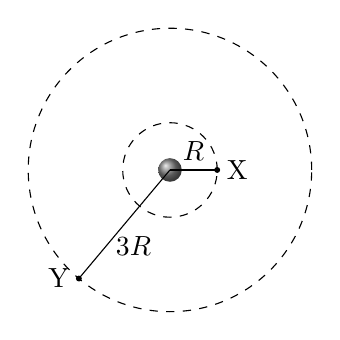
\begin{tikzpicture}[scale=.6]
      \tikzstyle{balloon}=[ball color=gray];
      \shade[balloon](0,0) circle(.25);
      \draw[dashed](0,0) circle(1);
      \draw[dashed](0,0) circle(3);
      \draw(0,0)--(1,0) node[pos=1,right]{X} node[midway,above]{$R$};
      \draw[fill=black](1,0) circle(.05);
      \begin{scope}[rotate=230]
        \draw(0,0)--(3,0) node[pos=1,left]{Y} node[pos=0.7,right]{$3R$};
        \draw[fill=black](3,0) circle(.05);
      \end{scope}
    \end{tikzpicture}
  \end{center}
  \begin{choices}
    \choice $a_X = 9a_Y$
    \choice $9a_X = a_Y$
    \choice $a_X = 3a_Y$
    \choice $3a_X = a_Y$
    \choice $a_X = a_Y$
  \end{choices}
    
  \question A satellite is in a stable circular orbit around the Earth at a
  radius $R$ and speed $v$. At what radius would the satellite travel in a
  stable orbit with a speed $2v$?
  \begin{choices}
    \choice $R/4$
    \choice $R/2$
    \choice $R$
    \choice $2R$
    \choice $4R$
  \end{choices}
  
  \question The Earth and the moon apply a gravitational force to each other.
  Which of the following statements is true?
  \begin{choices}
    \choice The Earth applies a greater force on the moon than the moon exerts
    on the Earth.
    \choice The Earth applies a smaller force on the moon than the moon exerts
    on the Earth.
    \choice The Earth applies a force on the moon, but the moon does not exert a
    force on the Earth.
    \choice The Earth does not apply a force on the moon, but the moon exerts a
    force on the Earth.
    \choice The force the Earth applies to the moon is equal and opposite to the
    force the moon applies to the Earth.
  \end{choices}
  \vspace{.7in}

  \question A planet orbits at a radius $R$ around a star of mass $M$. The
  period of orbit of the planet is
  \begin{choices}
    \choice $\sqrt{\dfrac{4\pi^2R^2}{GM}}$
    \choice $\dfrac{4\pi^2R^3}{GM}$
    \choice $\sqrt{\dfrac{4\pi^2R^3}{GM}}$
    \choice $\sqrt{\dfrac{4\pi^2R}{GM}}$
    \choice $\dfrac{GM}{4\pi^2R}$
  \end{choices}
  \newpage
  
  \question If a planet has twice the radius of Earth and half of Earth's
  density, what is the acceleration due to gravity on the surface of the planet
  (in terms of the gravitational acceleration $g$ on the surface of Earth)?
  \begin{choices}
    \choice $4g$
    \choice $2g$
    \choice $g$
    \choice $g/2$
    \choice $g/4$
  \end{choices}

  \question The graph below depicts the tangential velocities of several
  circular space stations with different radii. All the stations are spinning.
  Which of the following statements is true?
  \cpic{.44}{stations}
  \begin{choices}
    \choice The centripetal accelerations of the three shorter radii space
    stations are greater than \SI{10}{\metre\per\second\squared}; those of
    the larger ones are less than \SI{10}{\metre\per\second\squared}.
    \choice  The centripetal accelerations of the three shorter radii space
    stations are greater than \SI{5}{\metre\per\second\squared}; those of
      the larger ones are less than \SI{5}{\metre\per\second\squared}.
      \choice The centripetal accelerations of all the stations are all nearly
      \SI{5}{\metre\per\second\squared}.
      \choice The centripetal accelerations of all the stations are all nearly
      \SI{10}{\metre\per\second\squared}.
      \choice The centripetal accelerations of the three shorter radii space
      stations are less than \SI{10}{\metre\per\second\squared}; those of the
      larger ones are greater than \SI{10}{\metre\per\second\squared}.
  \end{choices}
  \newpage
  
  % THIS QUESTION IS FROM THE 2001 AP PHYSICS B FREE RESPONSE QUESTION #1
  \uplevel{
    \centering
    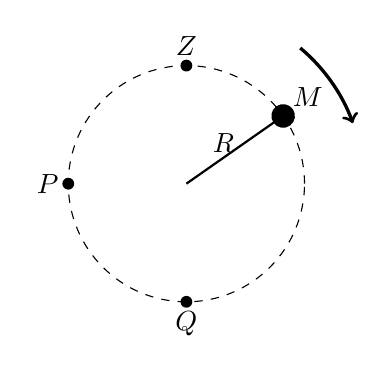
\begin{tikzpicture}[scale=.5]
      \draw[dashed](0,0) circle(3);
      \fill(-3,0) circle(.15) node[left]{$P$};
      \fill(0,-3) circle(.15) node[below]{$Q$};
      \fill(0,3) circle(.15) node[above]{$Z$};
      \draw[very thick,rotate=50,->](4.5,0) arc(0:-30:4.5);
      \begin{scope}[rotate=35]
        \draw[thick](0,0)--(3,0) node[pos=.6,left]{$R$};
        \fill(3,0) circle(.3) node[above right]{$M$};
      \end{scope}
    \end{tikzpicture}
  }

  \question A ball of mass $M$ is attached to a string of length $R$ and
  negligible mass. The ball moves clockwise in a vertical circle, as shown
  above. When the ball is at point $P$, the string is horizontal. Point $Q$ is
  at the bottom of the circle and point $Z$ is at the top of the circle. Air
  resistance is negligible. Express all algebraic answers in terms of the given
  quantities and fundamental constants.
  \begin{parts}
    \part On the figures below, draw and label all the forces exerted on the
    ball when it is at points $P$ and $Q$, respectively.
    \begin{center}
      \begin{tikzpicture}[scale=.6]
        \draw[dashed](0,0) circle(3);
        \fill(-3,0) circle(.25) node[left]{$P\;$};
        \draw[very thick,rotate=-75,->](3.5,0) arc(0:-30:3.5);
      \end{tikzpicture}
      \hspace{1in}
      \begin{tikzpicture}[scale=.6]
        \draw[dashed](0,0) circle(3);
        \fill(0,-3) circle(.25) node[above]{$Q$};
        \draw[very thick,rotate=-30,->](3.5,0) arc(0:-30:3.5);
      \end{tikzpicture}
    \end{center}

    \part Derive an expression for $v_\text{min}$, the minimum speed the ball
    can have at point $Z$ without leaving the circular path.
    
    \part The maximum tension the string can have without breaking is
    $T_\text{max}$. Derive an expression for $v_\text{max}$, the maximum speed
    the ball can have at point $Q$ without breaking the string.
    
    \part Suppose that the string breaks at the instant the ball is at point
    $P$. Describe the motion of the ball immediately after the string breaks.
  \end{parts}
  \newpage
  
  \question Two stars of equal mass $M$ are orbiting each other in a circular
  path. Show that the orbital period is given by:
  \begin{displaymath}
    T^2=\frac{2\pi^2d^3}{GM}
  \end{displaymath}
  where $d$ is the distance between the stars.
  \newpage
  
  \question Two stars of unequal mass orbit each other about their common
  center of mass as shown. The star of mass $M_1$ orbits in a circle of radius
  $r$, and the star of mass $M_2$ orbits in a circle of radius $2r$.
  \begin{center}
    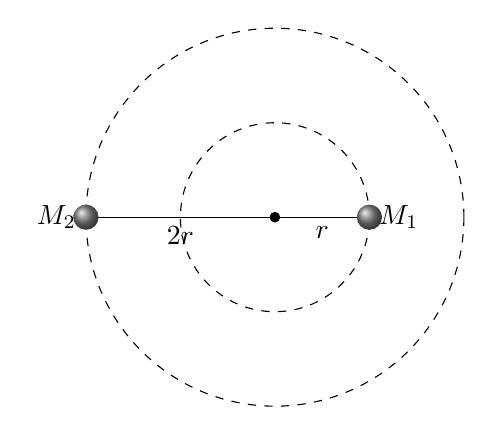
\begin{tikzpicture}[scale=.8]
      \tikzstyle{balloon}=[ball color=gray];
      \draw[fill=black](0,0) circle(.075);
      \draw[dashed](0,0) circle(3);
      \draw[dashed](0,0) circle(1.5);
      \draw[->](0,0)--(1.5,0) node[midway,below]{$r$};
      \shade[balloon] (1.5,0) circle (0.2) node[right]{$M_1$};
      \draw[->](0,0)--(-3,0) node[midway,below]{$2r$};
      \shade[balloon] (-3,0) circle (0.2) node[left]{$M_2$};
    \end{tikzpicture}
  \end{center}
  \begin{parts}
    \part Determine the ratio of masses $M_1/M_2$.

    \part Determine the ratio of the acceleration $a_1$ of $M_1$ to the
    acceleration $a_2$ of $M_2$.
    
    \part Determine the ratio of the period $T_1$ of $M _1$ to the period $T_2$
    of $M_2$.
  \end{parts}
  \newpage

  \question Two point particles of mass $m$ are on the $y$ axis at $y=a$ and
  $y=-a$, as shown in the figure below.
  \begin{center}
    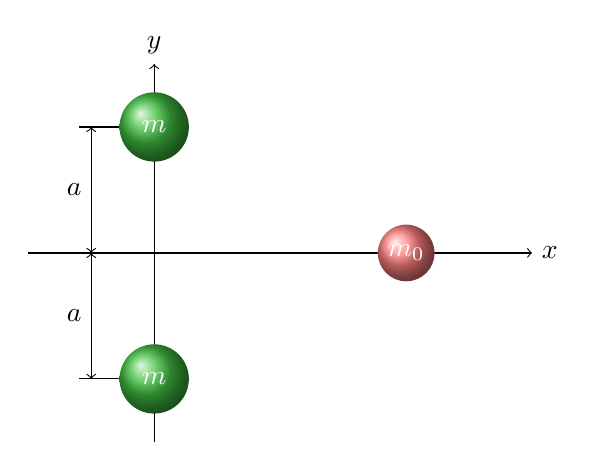
\begin{tikzpicture}[scale=.8]
      \tikzstyle{balloon1}=[ball color=green!50!gray];
      \tikzstyle{balloon2}=[ball color=red!50];
      \draw[->](-2,0)--(6,0) node[pos=1,right]{$x$};
      \draw[->](0,-3)--(0,3) node[pos=1,above]{$y$};
      \draw[<->](-1,0)--(-1,2) node[midway,left]{$a$};
      \draw[<->](-1,0)--(-1,-2)node[midway,left]{$a$};
      \draw(0,2)--(-1.2,2);
      \draw(0,-2)--(-1.2,-2);
      \shade[balloon1] (0,2) circle (.55) node[white]{$m$};
      \shade[balloon1] (0,-2)circle (.55) node[white]{$m$};
      \shade[balloon2] (4,0) circle (.45) node[white]{$m_0$};
    \end{tikzpicture}
  \end{center}
  \begin{parts}
    \part Derive the expression for the gravitational force exerted by these two
    particles on a third particle of mass $m_0$ located on the $x$ axis at a
    distance $x$ away from the origin.
    
    \part What is the gravitational field $\bm{g}$ on the $x$-axis due to the
    two particles?
    
    \part Show that $g_x$ (the $x$ component of $\bm{g}$) due to the two
    particles on the $y$ axis is approximately $-\dfrac{2Gm}{x^2}$
    when $x$ is much greater than $a$.
    
    \part (optional) Show that the maximum value of $|g_x|$ occurs at the point
    $x=\dfrac{\pm a}{\sqrt{2}}$.
  \end{parts}
  \newpage

  \uplevel{
    \centering
    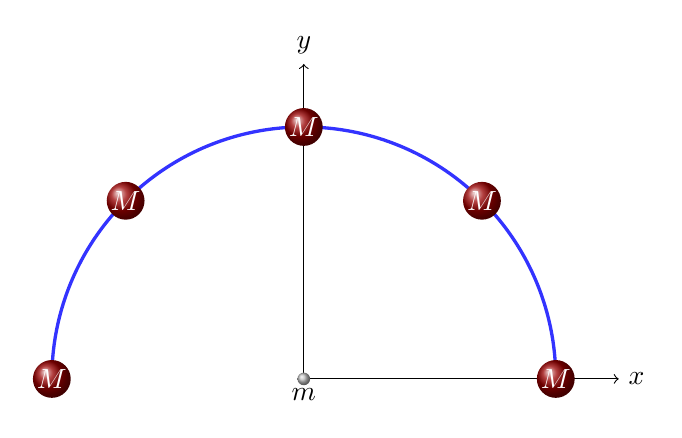
\begin{tikzpicture}[scale=.8]
      \tikzstyle{balloon1}=[ball color=gray!50];
      \tikzstyle{balloon2}=[ball color=red!60!black];
      \draw[->](0,0)--(5,0) node[pos=1,right]{$x$};
      \draw[->](0,0)--(0,5) node[pos=1,above]{$y$};
      \draw[very thick,blue!80](4,0) arc(0:180:4);
      \shade[balloon1] (0,0) circle (.1) node[below]{$m$};
      \foreach \theta in {0,45,...,180} {
        \begin{scope}[rotate=\theta]
          \shade[balloon2] (4,0) circle (.3) node[white]{$M$};
        \end{scope}
      }
    \end{tikzpicture}
  }
  \question Five equal masses $M$ are equally spaced on the arc of a semicircle
  of radius $R$ as shown in the figure below. A mass $m$ is located at the
  center of curvature of the arc. If $M$ is \SI{3}{\kilo\gram}, $m$ is
  \SI{21}{\kilo\gram}, and $R$ is \SI{10}{\centi\metre}, what is the force on
  $m$ due to the five masses?
\end{questions}
\end{document}
